\documentclass[pre,twocolumn,twoside,superscriptaddress,floatfix, aps, 10pt]{revtex4-1}

\usepackage{currfile}
\lefthyphenmin=3
\righthyphenmin=2

\usepackage{graphicx,epsfig,verbatim,enumerate}
\usepackage{amssymb,amsmath}
\usepackage{ifthen}

% Fonts and typesetting settings
\usepackage[sc]{mathpazo}
\usepackage[T1]{fontenc}
\linespread{1.05} % Palatino needs more space between lines
\usepackage{microtype}
\usepackage{textcomp}

\usepackage{longtable}

\usepackage{mathtools}

\newboolean{twocolswitch}

\newcommand{\www}[1]{\url{#1}}
\newcommand{\req}[1]{(\ref{#1})}
\newcommand{\Req}[1]{Eq.~(\ref{#1})}

% Lettrines
\usepackage{lettrine}

%useful shortcuts
\def\R{\ensuremath{\mathbb{R}}} %\ensuremath adds math mode, if forgotten
\def\Q{\ensuremath{\mathbb{Q}}}
\def\N{\ensuremath{\mathbb{N}}}
\def\Z{\ensuremath{\mathbb{Z}}}
\def\C{\ensuremath{\mathbb{C}}}

%shorcuts with arguments
\newcommand{\abs}[1]{\left\vert#1\right\vert} %nice absolute values
\newcommand{\bt}[1]{\textbf{#1}} %bold
\newcommand{\eq}[1]{\begin{align*}#1\end{align*}} %aligned equations
\newcommand{\norm}[1]{\left\lVert#1\right\rVert} %vector norm
\renewcommand{\eq}[1]{\begin{align*}#1\end{align*}} %aligned equations

%piecewise function

%\begin{displaymath}
%   f(x) = \left\{
%     \begin{array}{lr}
%       1 & : x \in \mathbb{Q}\\
%       0 & : x \notin \mathbb{Q}
%     \end{array}
%   \right.
%\end{displaymath} 


%environment
\newcommand{\tab}{\phantom{ssss}}


\usepackage{color}
\newcommand{\todo}[1]{\noindent\textcolor{blue}{{$\Box$ #1}}}

%colors
\definecolor{javagreen}{rgb}{0.25,0.5,0.35} %dark green color
\definecolor{lightblue}{rgb}{0.149,0.545,0.824} %solarized blue
\definecolor{sred}{rgb}{0.863, 0.196, 0.184} %solarized red

\newcommand{\blue}[1]{{\leavevmode\color{lightblue}{#1}}} %solarized blue 
\newcommand{\green}[1]{{\leavevmode\color{javagreen}{#1}}} %command for green
\newcommand{\red}[1]{{\leavevmode\color{sred}{#1}}} %solarized red
\newcommand{\gray}[1]{{\leavevmode\color[gray]{0.5}{#1}}} %gray text
\newcommand{\Prob}[1]{{\rm Pr}\left(#1\right)}


\setboolean{twocolswitch}{true}

\begin{document}

\title{\protect
Paper Template
}

\author{
\firstname{esteemed}
\surname{author}
}
\email{esteemed@mail.com}

\affiliation{Department of Magic,
    Hogwarts
  Burlington, VT 05401.}

\author{
\firstname{Alfred}
\surname{Dumbeldore}
}
\email{magic@uvm.edu}

\affiliation{Department of Mathemagi,
  Burlington, VT 05401.}

\author{
\firstname{Ernest}
\surname{Hemingway}
}
\email{letters_only@mail.com}

\affiliation{Department of Mysteries
    Ocean
}

\date{\today}

\begin{abstract}
  \protect
  this is the glorious abstract of abstractness summarizing methods,
  results, and contribution of paper our understanding of the world

 
\end{abstract}

\maketitle

\section*{Introduction}
Of Man's First Disobedience, and the Fruit... ~\cite{Milton1608}

\begin{figure*}[tp!]
  \centering	
  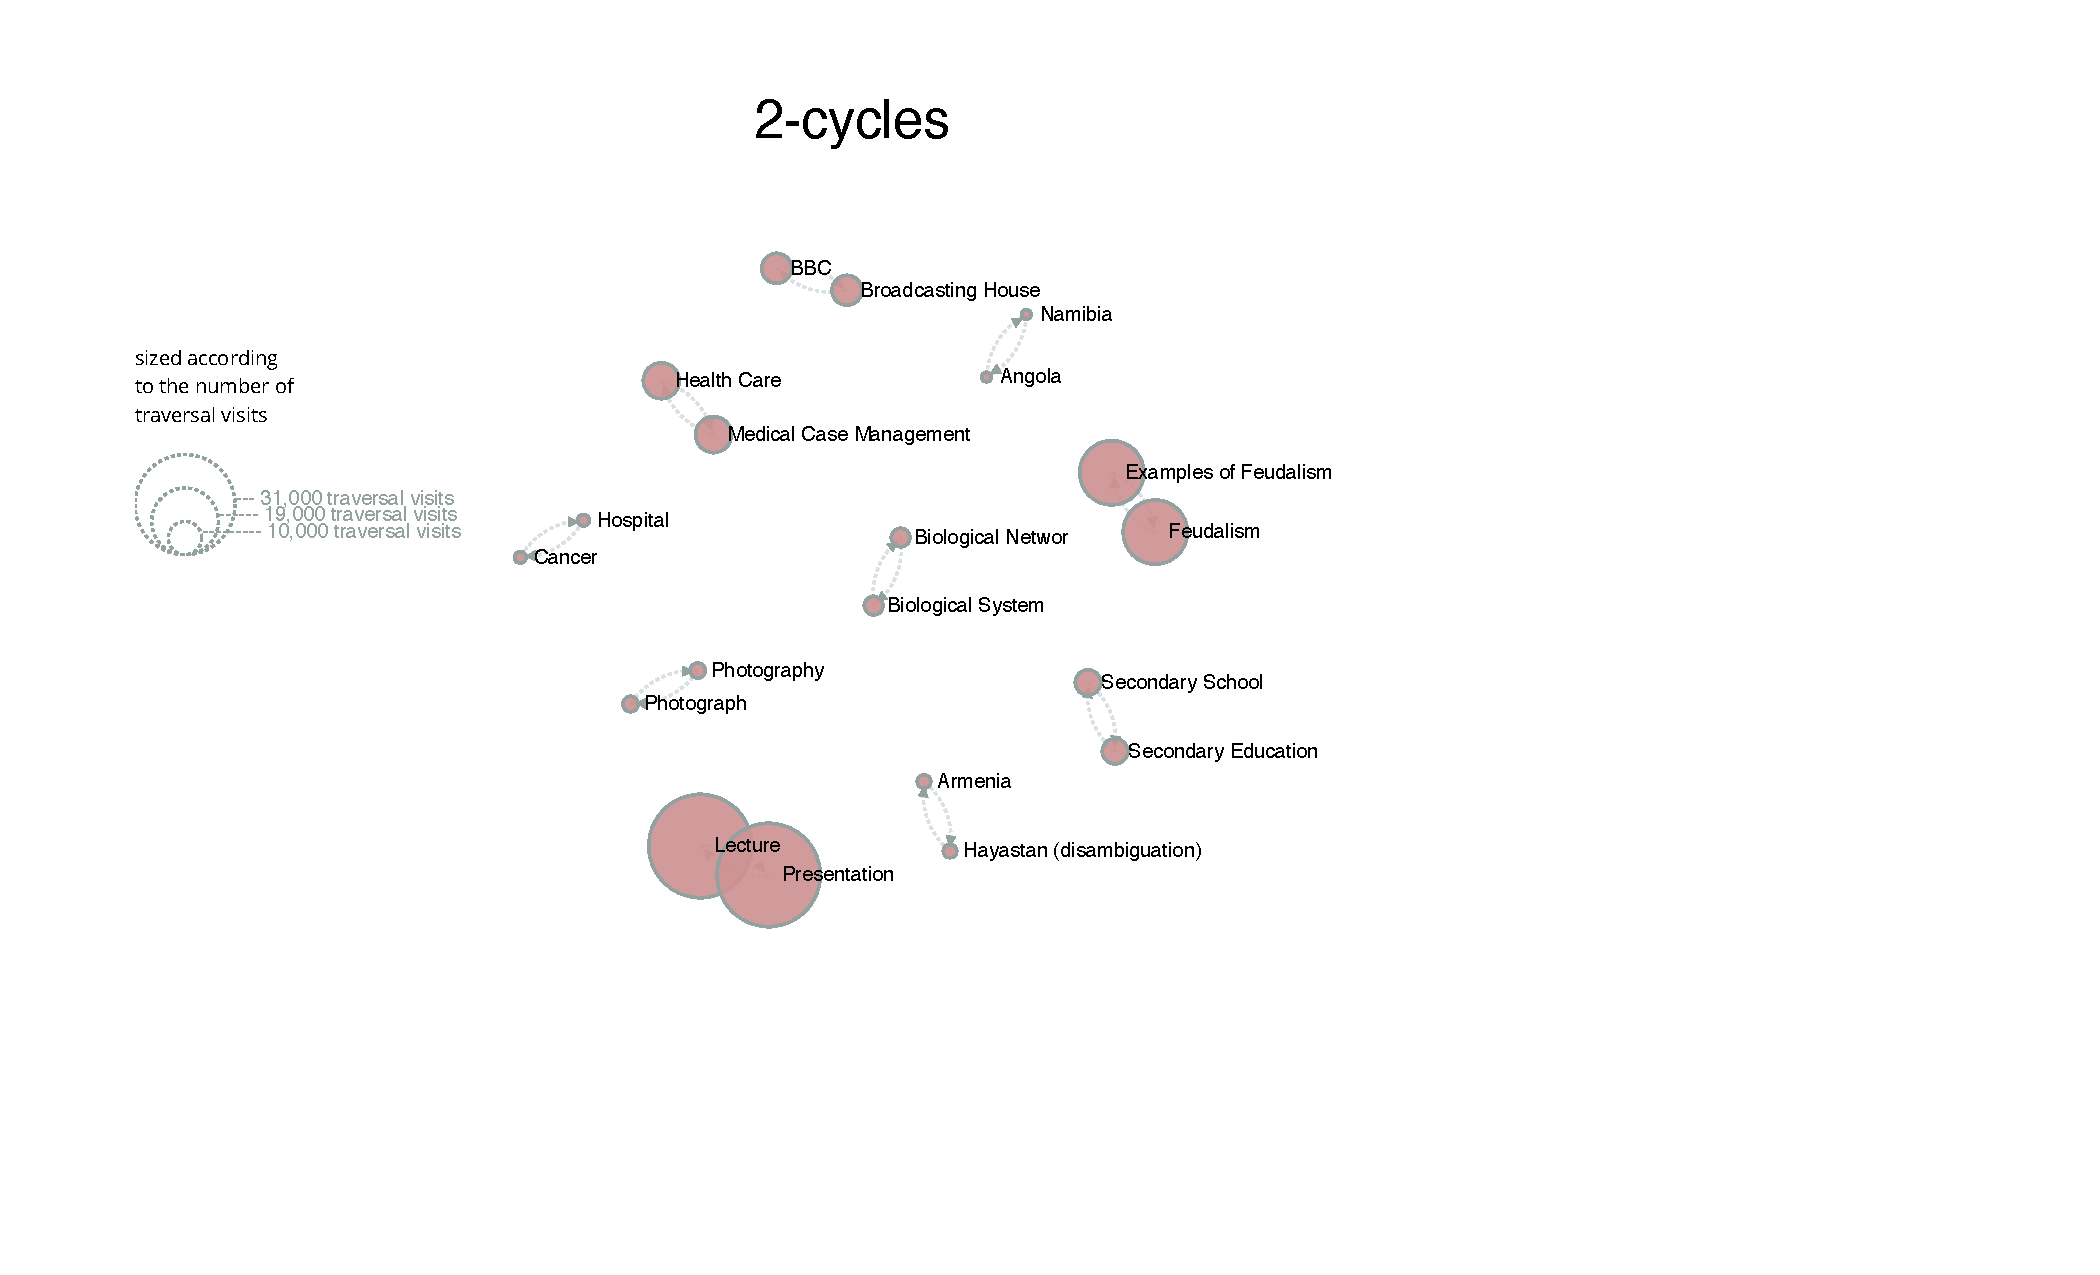
\includegraphics[width=\textwidth]{figures/2_cycles.pdf}  
  \caption{
    \textbf{title description}
    details details details
  }
  \label{fig:2 cycles}
\end{figure*}


\section*{Results and Discussion}
This is how you refrence a figure.~\ref{fig:2 cycles}

\section*{Methods}
insert urls like so:
\url{http://natsec.newamerica.net/} 

\acknowledgments
thank everyone


\begin{thebibliography}{15}%
\makeatletter
\providecommand \@ifxundefined [1]{%
 \@ifx{#1\undefined}
}%
\providecommand \@ifnum [1]{%
 \ifnum #1\expandafter \@firstoftwo
 \else \expandafter \@secondoftwo
 \fi
}%
\providecommand \@ifx [1]{%
 \ifx #1\expandafter \@firstoftwo
 \else \expandafter \@secondoftwo
 \fi
}%
\providecommand \natexlab [1]{#1}%
\providecommand \enquote  [1]{``#1''}%
\providecommand \bibnamefont  [1]{#1}%
\providecommand \bibfnamefont [1]{#1}%
\providecommand \citenamefont [1]{#1}%
\providecommand \href@noop [0]{\@secondoftwo}%
\providecommand \href [0]{\begingroup \@sanitize@url \@href}%
\providecommand \@href[1]{\@@startlink{#1}\@@href}%
\providecommand \@@href[1]{\endgroup#1\@@endlink}%
\providecommand \@sanitize@url [0]{\catcode `\\12\catcode `\$12\catcode
  `\&12\catcode `\#12\catcode `\^12\catcode `\_12\catcode `\%12\relax}%
\providecommand \@@startlink[1]{}%
\providecommand \@@endlink[0]{}%
\providecommand \url  [0]{\begingroup\@sanitize@url \@url }%
\providecommand \@url [1]{\endgroup\@href {#1}{\urlprefix }}%
\providecommand \urlprefix  [0]{URL }%
\providecommand \Eprint [0]{\href }%
\providecommand \doibase [0]{http://dx.doi.org/}%
\providecommand \selectlanguage [0]{\@gobble}%
\providecommand \bibinfo  [0]{\@secondoftwo}%
\providecommand \bibfield  [0]{\@secondoftwo}%
\providecommand \translation [1]{[#1]}%
\providecommand \BibitemOpen [0]{}%
\providecommand \bibitemStop [0]{}%
\providecommand \bibitemNoStop [0]{.\EOS\space}%
\providecommand \EOS [0]{\spacefactor3000\relax}%
\providecommand \BibitemShut  [1]{\csname bibitem#1\endcsname}%
\let\auto@bib@innerbib\@empty
%</preamble>

\bibitem [{\citenamefont {Milton}(1608)}]{Milton1608}%
  \BibitemOpen
  \bibfield  {author} {\bibinfo {author} {\bibfnamefont {L.~F.}\ \bibnamefont
  {Milton}},\ }\href@noop {} {\bibfield  {journal} {\bibinfo  {journal}
  {Journal of 1600s Paper}\ }\textbf {\bibinfo
  {volume} {43}},\ \bibinfo {pages} {523} (\bibinfo {year} {1608})}\BibitemShut
  {NoStop}%
\bibitem [{\citenamefont {Morgenstern}\ \emph {et~al.}(2013)\citenamefont
  {Morgenstern}, \citenamefont {Velasquez}, \citenamefont {Manrique},
  \citenamefont {Hong}, \citenamefont {Johnson},\ and\ \citenamefont
  {Johnson}}]{Morgenstern2013}%
\end{thebibliography}%

\clearpage

\end{document}
